\documentclass[conference]{IEEEtran}
\usepackage{amsmath,amssymb}
\usepackage{graphicx}
\usepackage{booktabs}
\usepackage{listings}
\usepackage{xcolor}
\usepackage{cite}
\usepackage[hidelinks]{hyperref}
\lstset{basicstyle=\ttfamily\scriptsize,breaklines=true,frame=single,columns=fullflexible}
\begin{document}
\title{Reproducing INSIDE: EigenScore and Test-Time Feature Clipping for LLM Hallucination Detection}
\author{\IEEEauthorblockN{Aayaan Ali Khan}\IEEEauthorblockA{ID: 202411001}
\and\IEEEauthorblockN{Shlok Bhavsar}\IEEEauthorblockA{ID: 202411018}
\and\IEEEauthorblockN{Prapti Chotaliya}\IEEEauthorblockA{ID: 202411030}}
\maketitle
\begin{abstract}
We reproduce the method of \emph{INSIDE: LLMs' Internal States Retain the Power of Hallucination Detection} (Chen et al., ICLR 2024). The paper proposes two components: \emph{EigenScore}, a hallucination score computed from the covariance of sentence embeddings taken from the middle layer of a language model, and \emph{test-time feature clipping}, which truncates extreme activations of the penultimate layer. The authors' public repository could not be executed as released, and it does not contain the feature-clipping component at all. We repaired twelve blocking defects, implemented feature clipping from the paper's description, added support for running a 7B model on an 8~GB GPU, and wrote an automated test suite. We then evaluated on 250 CoQA questions using Llama-2-7B in 4-bit precision. The ordering of the five detection methods reported in the paper is reproduced exactly, with EigenScore best (AUROC 83.5 without and 82.5 with clipping). The effect of feature clipping could not be resolved at this sample size: a paired bootstrap gives a change of $-1.0$ points with a 95\% interval of $[-4.7,+2.6]$.
\end{abstract}
\begin{IEEEkeywords}hallucination detection, large language models, EigenScore, feature clipping, reproducibility\end{IEEEkeywords}
\section{Introduction}
Large language models (LLMs) frequently produce fluent but factually incorrect statements, commonly called \emph{hallucinations}. Detecting such outputs without external fact-checking is important for deployment. Existing approaches operate either on token probabilities (perplexity, entropy) or on the decoded text (agreement between several sampled answers). Both discard information that is still present inside the network.

The selected paper, INSIDE~\cite{chen2024inside}, instead measures the disagreement among several sampled answers \emph{in the model's internal embedding space}. This report documents our implementation and reproduction of that work for the course CS367. Our contributions are:
\begin{enumerate}
  \item A working, documented version of the authors' code base (twelve blocking defects repaired).
  \item An implementation of test-time feature clipping (Section~3.2 of the paper), which is absent from the public repository.
  \item Memory engineering that allows the pipeline to run on a consumer GPU with 8~GB of memory.
  \item An automated test suite of eight tests.
  \item An experimental reproduction on CoQA, with statistical analysis of the results.
\end{enumerate}

%--------------------------------------------------------------------
\section{The Method}
\subsection{EigenScore}
For a question $x$, the model is sampled $K$ times, producing responses $y_1,\dots,y_K$. For each response, the sentence embedding $z_i\in\mathbb{R}^d$ is the hidden state of the last generated token at the middle layer. Let $Z=[z_1,\dots,z_K]\in\mathbb{R}^{d\times K}$ and let $J_d=I_d-\tfrac1d\mathbf{1}\mathbf{1}^\top$ be the centering matrix. The covariance matrix is
\begin{equation}
\Sigma = Z^\top J_d Z \in \mathbb{R}^{K\times K},
\end{equation}
and the EigenScore is
\begin{equation}
\mathcal{E}(Y\mid x,\theta)=\frac1K\log\det(\Sigma+\alpha I_K)=\frac1K\sum_{i=1}^{K}\log\lambda_i,
\end{equation}
where $\lambda_i$ are the eigenvalues of $\Sigma+\alpha I_K$ and $\alpha=10^{-3}$ is a regulariser that keeps the matrix full rank. Up to additive constants this quantity is the differential entropy of a Gaussian fitted to the embeddings. If the model is confident, the $K$ embeddings nearly coincide, most eigenvalues collapse to the floor $\alpha$, and the score is low. If the model is guessing, the embeddings spread out and the score is high. A larger score therefore indicates a more probable hallucination.

\subsection{Test-time feature clipping}
Self-consistent hallucinations, where the model repeats the same wrong answer, are invisible to any consistency measure. The paper hypothesises that extreme activations in the penultimate layer contribute to such overconfidence and truncates them elementwise:
\begin{equation}
\mathrm{FC}(h)=\begin{cases}
h_{\min}, & h<h_{\min}\\
h, & h_{\min}\le h\le h_{\max}\\
h_{\max}, & h>h_{\max}
\end{cases}
\end{equation}
The thresholds $h_{\min}$ and $h_{\max}$ are the bottom and top $p$-th percentiles of each neuron, estimated from a memory bank of the most recent $N$ token activations. The paper uses $p=0.2\%$ and $N=3000$.

\subsection{Baselines and evaluation}
We compare against the paper's four baselines: \emph{Perplexity}, \emph{Length-Normalised Entropy} (LN-Entropy), \emph{Lexical Similarity} (mean pairwise ROUGE-L between the $K$ answers) and \emph{Energy}. A response is labelled correct when its ROUGE-L against the reference answer exceeds $0.5$ (the paper's $\mathrm{AUC}_r$). Methods are compared by the area under the ROC curve (AUROC) of the score as a predictor of incorrectness.

%--------------------------------------------------------------------
\section{Implementation}
\subsection{State of the original code}
The released repository (\texttt{alibaba/eigenscore}, commit \texttt{ea8062a}) has empty setup and run sections and could not be executed. Table~\ref{tab:bugs} lists the blocking defects we repaired. Every original file is preserved next to the repaired one with the suffix \texttt{.orig}.

\begin{table*}[t]
\centering\small
\caption{Blocking defects in the released code and their repairs.}\label{tab:bugs}
\begin{tabular}{@{}rp{3.6cm}p{6.4cm}p{5.6cm}@{}}
\toprule
\# & File & Problem & Repair\\
\midrule
1 & \texttt{pipeline/generate.py} & Imports non-existent module \texttt{dataeval.TruthfulQA} & Import removed\\
2 & \texttt{func/metric.py} & \texttt{np.float} (removed in NumPy 1.24) used 14 times & Replaced by \texttt{np.float64}\\
3 & \texttt{\_settings.py} & Absolute paths of the authors' machine & Repository-relative, overridable by environment variables\\
4 & \texttt{pipeline/generate.py} & Log opened before its directory exists & Directory created first\\
5 & \texttt{func/evalFunc.py} & Imports only valid from inside \texttt{func/} & Package-qualified imports\\
6 & \texttt{func/metric.py} & \texttt{selfcheckgpt} imported at load time, used by dead code & Import moved into the function\\
7 & \texttt{pipeline/generate.py} & BERTScore model built from a missing local path for a disabled metric & Construction removed\\
8 & \texttt{dataeval/*} & \texttt{import ipdb} at module level & Commented out\\
9 & \texttt{func/plot.py} & Saves to a missing directory, then blocks on \texttt{plt.show()} & \texttt{Agg} backend, \texttt{makedirs}, no \texttt{show()}\\
10 & \texttt{func/evalFunc.py} & \texttt{split("\_")[1]} fails for ordinary paths & Whole path passed on\\
11 & \texttt{func/metric.py} & \texttt{.to("cuda")} hard-coded 16 times & Device derived from the tensors\\
12 & \texttt{dataeval/load.py} & \texttt{DEFAULT\_DEVICE='cuda:7'} & Left unchanged (off the execution path)\\
\bottomrule
\end{tabular}
\end{table*}

An additional defect was found at run time. When generations were split into several forward passes, the original code recomputed EigenScore inside the batch loop, so only the last batch (2 of the 10 answers) contributed. We pool the embeddings of all batches before forming the covariance matrix; a test confirms equivalence with the original function in the single-batch case.

\subsection{Feature clipping}
The module \texttt{func/feature\_clip.py} implements Section 3.2 of the paper. The class \texttt{FeatureClipper} maintains a ring buffer of $N$ token activations, computes per-neuron percentile thresholds, and applies Equation~(3). It is attached as a forward hook on the penultimate decoder layer, so that the clipping acts during autoregressive decoding and influences the generated text. Until the bank holds a minimum number of rows the hook is a pass-through, so thresholds are never estimated from a few tokens.

\subsection{Running a 7B model on an 8~GB GPU}
\begin{itemize}
  \item \textbf{4-bit weights} (NF4, \texttt{bitsandbytes}): a 7B model needs about 3.9~GB instead of 13.5~GB.
  \item \textbf{\texttt{--num\_return\_sequences}}: the $K=10$ samples are produced in several smaller forward passes, keeping the paper's value of $K$.
  \item \textbf{\texttt{--low\_memory}}: requesting all hidden states retains every layer for every token, which ran out of memory on long CoQA stories. Because EigenScore reads only one layer, a forward hook captures only the middle layer. A test verifies the result is identical to the full path.
\end{itemize}

\subsection{Tests}
The file \texttt{tests/test\_setup.py} contains eight tests, all of which pass: imports; clip thresholds agree with \texttt{numpy.percentile}; clipping implements Equation~(3); ring-buffer wrap-around and warm-up; pooled EigenScore equals the original function; EigenScore separates consistent from diverse responses; the low-memory path equals the full-hidden-state path; decoder-layer discovery.

%--------------------------------------------------------------------
\section{Experimental Setup}
\begin{table}[t]
\centering\small
\caption{Our setup compared with the paper's.}
\begin{tabular}{@{}p{1.6cm}p{2.9cm}p{3.0cm}@{}}
\toprule
 & Paper & This work\\
\midrule
Model & LLaMA-7B (fp16) & Llama-2-7B (4-bit NF4)\\
Dataset & CoQA, 7983 pairs & CoQA, 250 questions\\
Hardware & --- & NVIDIA RTX 4060 Laptop, 8~GB\\
$K$ / temperature / top-$p$ & 10 / 0.5 / 0.99 & 10 / 0.5 / 0.99\\
top-$k$ & 5 & 10 (repository default)\\
$\alpha$ / $p$ / $N$ & $10^{-3}$ / 0.2\% / 3000 & $10^{-3}$ / 0.2\% / 3000\\
Embedding & middle layer, last token & middle layer, last token\\
Correctness & ROUGE-L ($\mathrm{AUC}_r$) and sentence similarity ($\mathrm{AUC}_s$) & ROUGE-L ($\mathrm{AUC}_r$) only\\
\bottomrule
\end{tabular}
\end{table}
The deviations are forced by the 8~GB GPU and by the unavailability of the \texttt{nli-roberta-large} model, which is needed for $\mathrm{AUC}_s$. The claim tested is therefore the \emph{ordering} of the methods, not the exact numbers. The model answered 36.8\% of the 250 questions correctly. Two runs were made with an identical seed (2023) and identical questions: one without and one with feature clipping.

\begin{lstlisting}
python -m pipeline.generate --model llama2-7b-hf --dataset coqa \
    --load_in_4bit --low_memory --feature_clip --no_sentsim \
    --num_generations_per_prompt 10 --num_return_sequences 2 \
    --fraction_of_data_to_use 0.03132 --seed 2023 --project_ind 10
python -m func.evalFunc data/output/llama2-7b-hf_coqa_10/0.pkl --correctness rouge
\end{lstlisting}

%--------------------------------------------------------------------
\section{Results}
\subsection{Comparison of detection methods}
\begin{table}[t]
\centering
\caption{AUROC (\%) on 250 CoQA questions, $\mathrm{AUC}_r$. The paper's column is LLaMA-7B, Table~1.}\label{tab:auroc}
\begin{tabular}{@{}lccc@{}}
\toprule
Method & Paper & This work & This work $+$FC\\
\midrule
Energy & 54.7 & 54.7 & 53.1\\
Perplexity & 68.3 & 72.3 & 71.4\\
LN-Entropy & 73.6 & 77.5 & 77.3\\
Lexical Similarity & 77.8 & 80.5 & 79.3\\
\textbf{EigenScore} & \textbf{80.8} & \textbf{83.5} & 82.5\\
\bottomrule
\end{tabular}
\end{table}
The ranking EigenScore $>$ Lexical Similarity $>$ LN-Entropy $>$ Perplexity $>$ Energy is identical to the paper's. Energy, an out-of-distribution detector not designed for this task, is close to chance.

The paper's EigenScore figure of 80.8 already includes feature clipping (its Table~2 reports 79.3 without and 80.4 with clipping in $\mathrm{AUC}_s$), whereas its baselines are without clipping. The like-for-like comparison for 80.8 is therefore our clipped run, 82.5.

\begin{figure}[t]
\centering
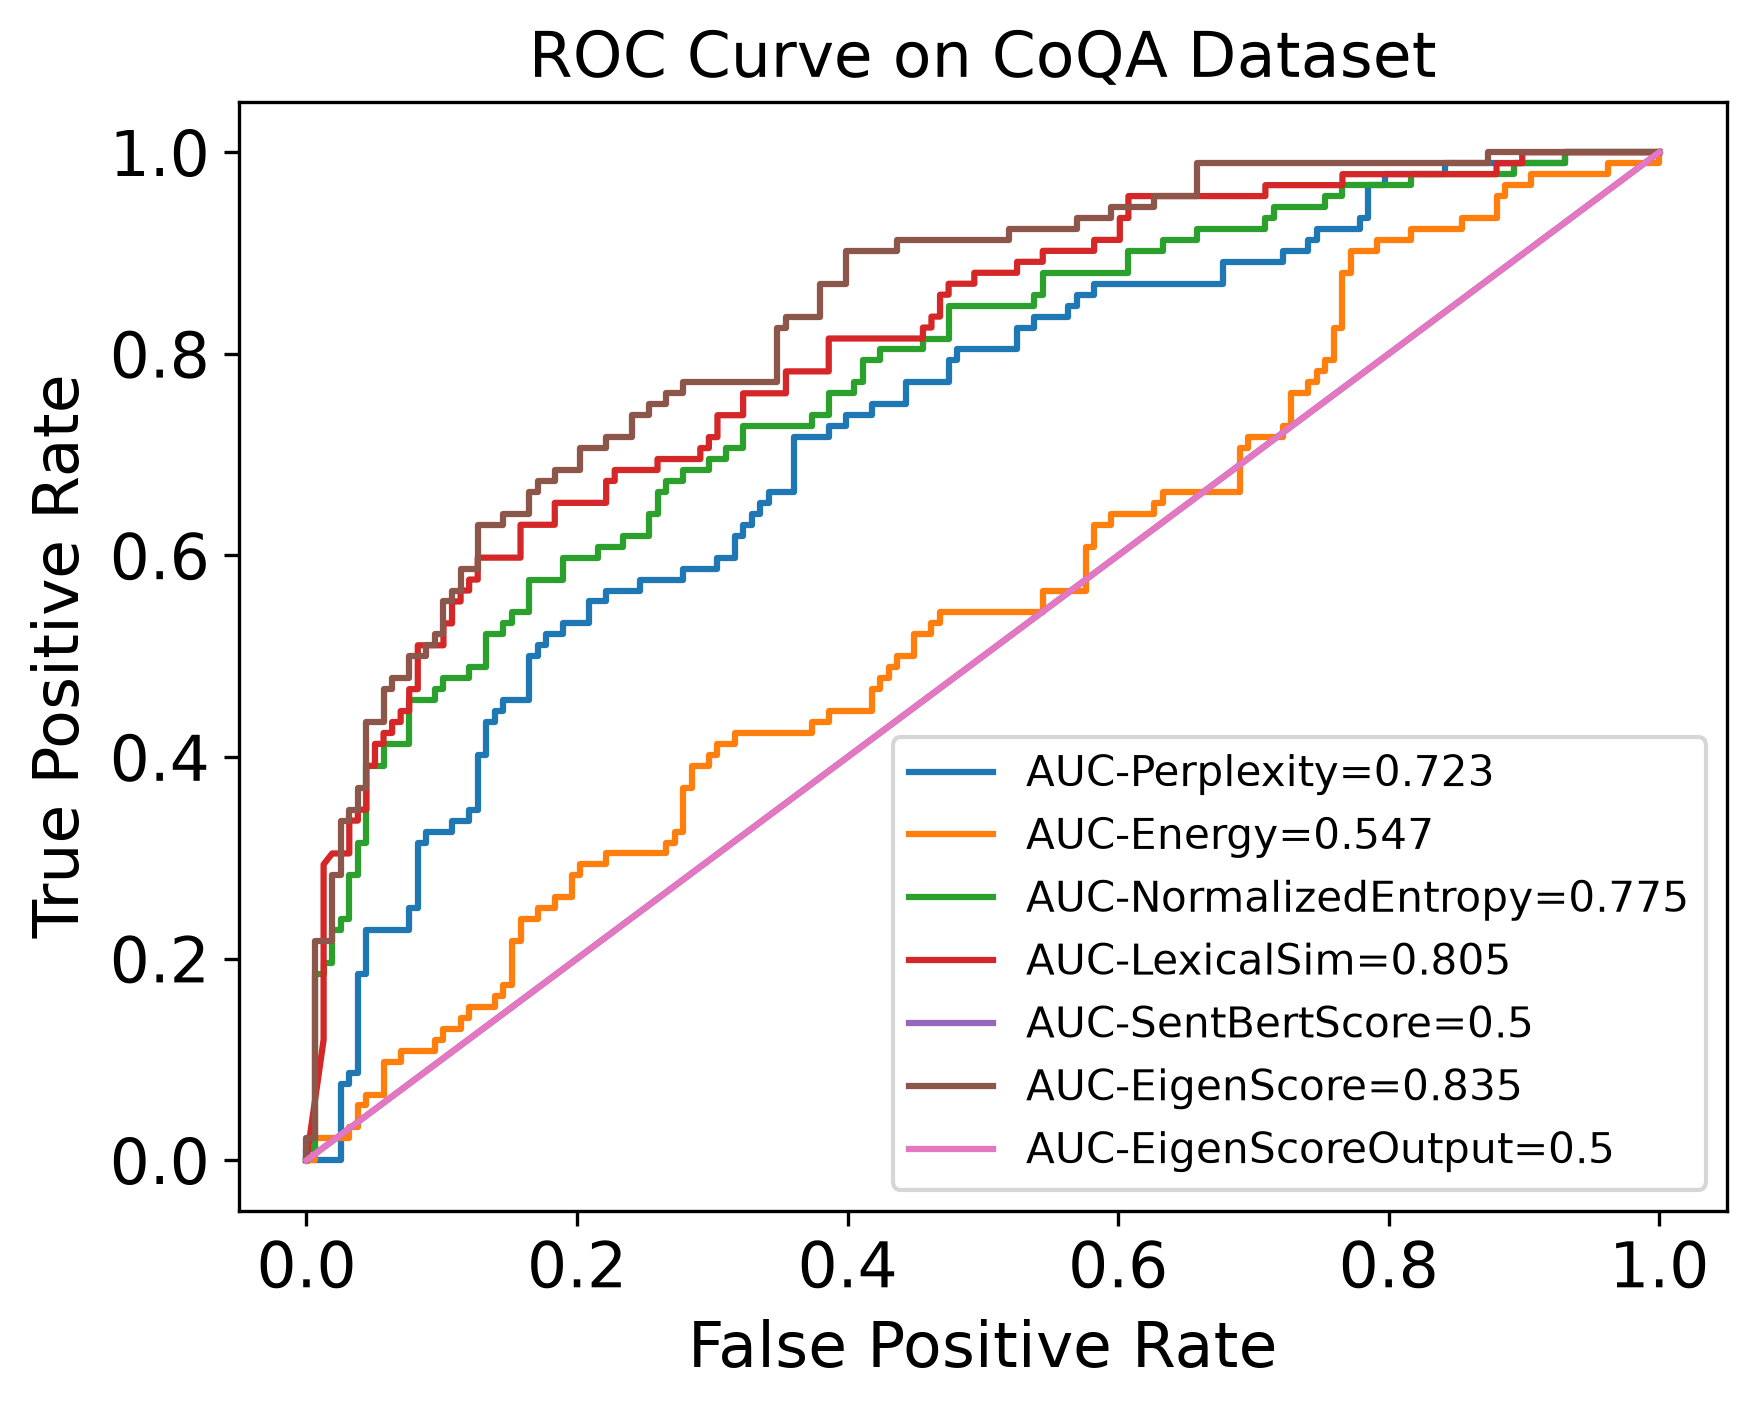
\includegraphics[width=0.95\columnwidth]{figures/auroc_nofc.png}
\caption{ROC curves on CoQA, without feature clipping. The entries ``SentBertScore'' and ``EigenScoreOutput'' are placeholders at 0.5 because the sentence-similarity model was not used.}
\end{figure}
\begin{figure}[t]
\centering
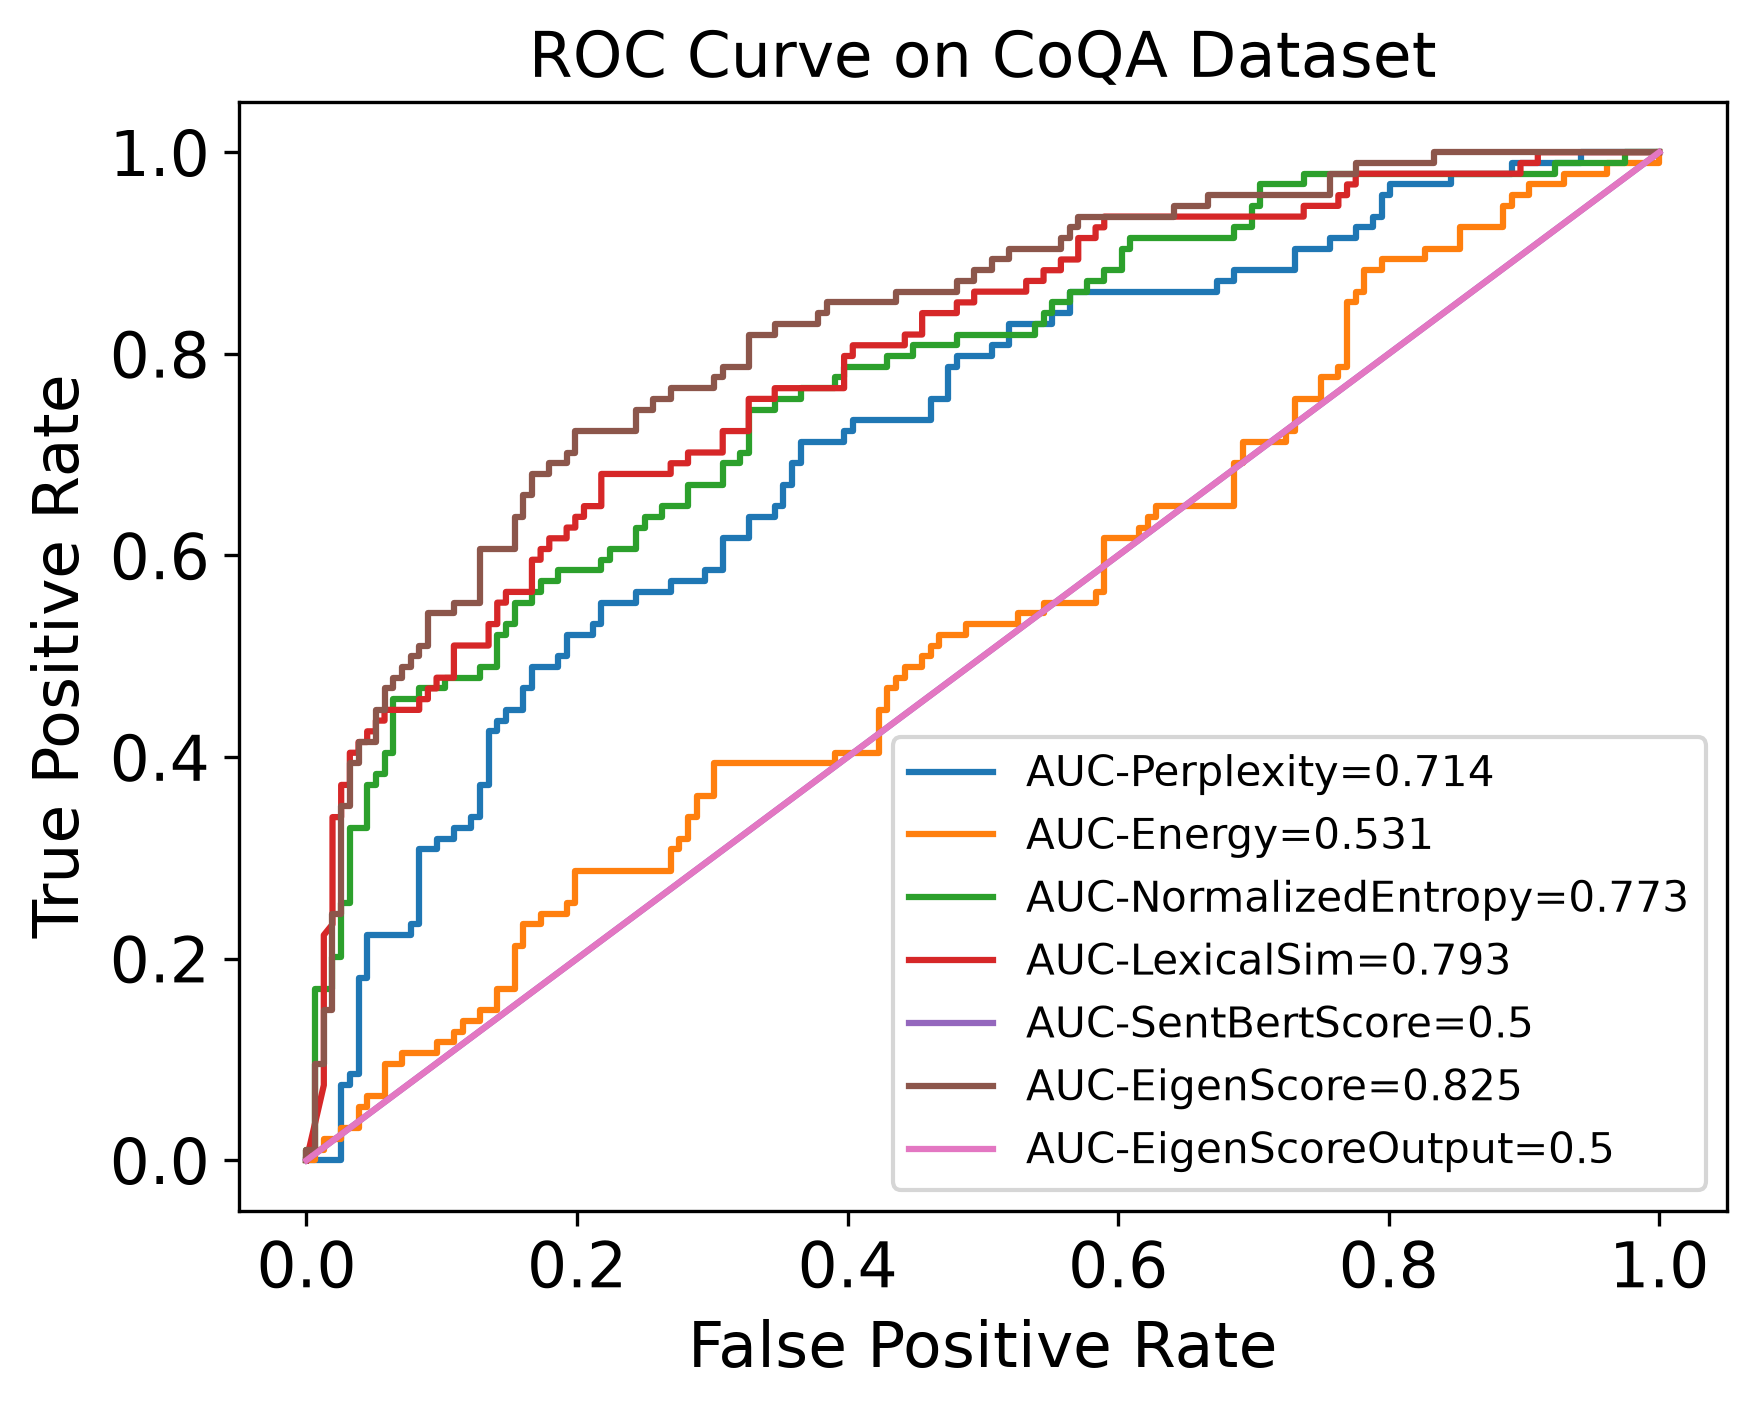
\includegraphics[width=0.95\columnwidth]{figures/auroc_fc.png}
\caption{ROC curves on CoQA, with feature clipping.}
\end{figure}

\subsection{EigenScore against the strongest baseline}
A paired bootstrap over questions gives
\begin{equation*}
\begin{aligned}\Delta\mathrm{AUROC}&=+0.0293,\\ 95\%\ \mathrm{CI}&=[-0.0057,+0.0651],\\ P(>0)&=0.95.\end{aligned}
\end{equation*}
This agrees in sign and magnitude with the paper's advantage of about $+3$ points on CoQA, and falls just short of excluding zero at 250 questions.

\subsection{Feature clipping}
The paper reports that clipping improves EigenScore on CoQA by $+1.1$ points ($\mathrm{AUC}_s$). We measured a change of
\begin{equation*}
\begin{aligned}\Delta\mathrm{AUROC}&=-0.0102,\\ 95\%\ \mathrm{CI}&=[-0.0468,+0.0263],\\ P(\text{FC helps})&=0.30\end{aligned}
\end{equation*}
(10\,000 paired bootstrap resamples, identical questions and seed). The interval contains both zero and the paper's $+0.011$, so our experiment neither confirms nor contradicts the claim; it lacks the resolution to do so. The paper used 7983 questions. Clipping was verifiably active: 13\,749\,839 activations were clipped out of $1\,159\,186\times4096$, i.e.\ 0.29\% (at most about 0.4\% is expected from $p=0.2\%$ per tail), and the thresholds are unit-tested against \texttt{numpy.percentile}. We also measured $\mathrm{AUC}_r$ where the paper reports $\mathrm{AUC}_s$, so the two quantities are not strictly the same.

%--------------------------------------------------------------------
\section{Discussion and Limitations}
\begin{itemize}
  \item \textbf{Sample size.} 250 questions give confidence intervals of roughly $\pm4$ points; effects of about one point cannot be resolved. A full run (\texttt{--fraction\_of\_data\_to\_use 1}) takes about 13 hours per configuration on our GPU.
  \item \textbf{Model and precision.} Llama-2-7B in 4 bits differs from the paper's LLaMA-7B in fp16, so absolute values are not directly comparable.
  \item \textbf{Correctness measure.} Only ROUGE-L correctness was evaluated. The EigenScore-Output baseline and $\mathrm{AUC}_s$ require \texttt{nli-roberta-large}, which was unavailable.
  \item \textbf{Sampling.} Top-$k$ was 10 rather than the paper's 5.
  \item \textbf{Logarithm base.} The authors' code uses $\log_{10}$ where Equation~(2) writes $\log$. This is a constant factor and cannot change AUROC or the sign of correlations; we left it unchanged to match published numbers.
  \item \textbf{Inherent limits of the method.} It requires access to internal states (so not black-box APIs), costs $K$ generations per query, and detects but does not correct hallucinations.
\end{itemize}

%--------------------------------------------------------------------
\section{Conclusion}
We obtained a working implementation of the INSIDE method, including the feature-clipping component that the authors' repository lacks, and reproduced the paper's central empirical finding: the relative ordering of the five hallucination detectors, with EigenScore the strongest. The additional claim that feature clipping improves EigenScore could not be tested conclusively with our compute budget; the implementation is verified by tests and shown to be active, and a full-scale run is the natural next step.

%--------------------------------------------------------------------

\section{Submission Contents}
\begin{lstlisting}
CS367_Submission/
  report/report.pdf, report.tex     this document
  INSIDE_paper_...pdf               the original paper
  source_code/
    pipeline/generate.py            sampling + score computation
    func/metric.py                  EigenScore and baselines
    func/feature_clip.py            feature clipping (new)
    func/evalFunc.py, plot.py       evaluation, ROC plots
    models/, dataeval/, utils/      model loading, datasets
    tests/test_setup.py             8 automated tests
    data/output/                    raw results (.pkl), logs, figures
    README.md, CHANGES.md, RESULTS.md, requirements.txt, run.sh
\end{lstlisting}

\section{Reproduction Instructions}
\begin{lstlisting}
cd source_code
uv venv --python 3.11 .venv && source .venv/bin/activate
uv pip install torch --index-url https://download.pytorch.org/whl/cu124
uv pip install -r requirements.txt
python -m tests.test_setup                # 8/8 should pass
bash run.sh                               # generation + evaluation
\end{lstlisting}
A CUDA GPU is required. CoQA and SQuAD are public datasets and must be placed under \texttt{data/datasets/} (\texttt{coqa-dev-v1.0.json}, \texttt{dev-v2.0.json}); they are omitted from the submission to keep it small.


\begin{thebibliography}{1}
\bibitem{chen2024inside} C.~Chen, K.~Liu, Z.~Chen, Y.~Gu, Y.~Wu, M.~Tao, Z.~Fu, and J.~Ye, ``INSIDE: LLMs' internal states retain the power of hallucination detection,'' in \emph{Proc. ICLR}, 2024. [Online]. Available: https://arxiv.org/abs/2402.03744
\bibitem{code} ``alibaba/eigenscore.'' [Online]. Available: https://github.com/alibaba/eigenscore
\end{thebibliography}
\end{document}
